\documentclass{article}
\usepackage[paperletter]{geometry}
\geometry{top=1.0in, bottom=1.0in, left=1.0in, right=1.0in}
\usepackage[utf8]{inputenc}
\usepackage{cancel}
\usepackage{tikz}
\usepackage{siunitx}
\usepackage{amsmath}
\usepackage{mathdots}
\usepackage{yhmath}
\usepackage{color}
\usepackage{array}
\usepackage{multirow}
\usepackage{amssymb}
\usepackage{gensymb}
\usepackage{tabularx}
\usepackage{booktabs}
\usepackage{booktabs}
\usepackage{float}
\usepackage{multicol}
\usetikzlibrary{fadings}
\usetikzlibrary{patterns}
\usetikzlibrary{shadows.blur}
\usepackage[symbol]{footmisc}
\renewcommand*{\thefootnote}{\fnsymbol{footnote}}
\usepackage{everysel}
\usepackage{ragged2e}
\renewcommand*\familydefault{\ttdefault}
\EverySelectfont{%
\fontdimen2\font=0.4em% interword space
\fontdimen3\font=0.2em% interword stretch
\fontdimen4\font=0.1em% interword shrink
\fontdimen7\font=0.1em% extra space
\hyphenchar\font=`\-% to allow hyphenation
}
\pagenumbering{gobble}
\title{Determining the Spring Constant Lab \\ AP \textsc{Physics} $-$ 1}
\author{Michael \textsc{Brodskiy}}
\date{March 2, 2020}

\begin{document}

\maketitle
\begin{center}
\begin{tabular}{l r}
\underline{Date Performed}: & February 25, 2020 \\\\ % Date the experiment was performed
\underline{Partners}: & Alden Woronicz \\ & Al McLeroy \\\\
\underline{Instructor}: & Mrs. Halle \\\\\\\\\\ % Instructor/supervisor
\end{tabular}
\end{center}
\newpage
    
\section{Finding the Spring Constant}

\subsection{Method 1}

\begin{figure}[H]
    

\begin{center}
\tikzset{every picture/.style={line width=0.75pt}} %set default line width to 0.75pt        

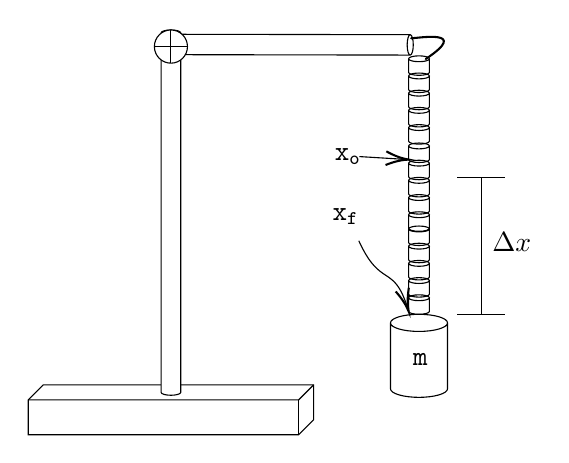
\begin{tikzpicture}[x=0.75pt,y=0.75pt,yscale=-1,xscale=1]
%uncomment if require: \path (0,300); %set diagram left start at 0, and has height of 300

%Shape: Cube [id:dp3909284610505568] 
\draw   (82,248.2) -- (89.2,241) -- (219.5,241) -- (219.5,257.8) -- (212.3,265) -- (82,265) -- cycle ; \draw   (219.5,241) -- (212.3,248.2) -- (82,248.2) ; \draw   (212.3,248.2) -- (212.3,265) ;
%Shape: Can [id:dp981667617906977] 
\draw  [fill={rgb, 255:red, 255; green, 255; blue, 255 }  ,fill opacity=1 ] (155.5,71.43) -- (155.5,244.58) .. controls (155.5,245.36) and (153.37,246) .. (150.75,246) .. controls (148.13,246) and (146,245.36) .. (146,244.58) -- (146,71.43) .. controls (146,70.64) and (148.13,70) .. (150.75,70) .. controls (153.37,70) and (155.5,70.64) .. (155.5,71.43) .. controls (155.5,72.21) and (153.37,72.85) .. (150.75,72.85) .. controls (148.13,72.85) and (146,72.21) .. (146,71.43) ;
%Shape: Can [id:dp04414332644892305] 
\draw  [fill={rgb, 255:red, 255; green, 255; blue, 255 }  ,fill opacity=1 ] (266.03,82.1) -- (150.82,81.9) .. controls (150.01,81.9) and (149.35,79.7) .. (149.36,76.99) .. controls (149.36,74.28) and (150.02,72.08) .. (150.84,72.08) -- (266.05,72.28) .. controls (266.86,72.28) and (267.52,74.48) .. (267.51,77.19) .. controls (267.51,79.91) and (266.85,82.1) .. (266.03,82.1) .. controls (265.22,82.1) and (264.56,79.9) .. (264.57,77.19) .. controls (264.57,74.48) and (265.24,72.28) .. (266.05,72.28) ;
%Flowchart: Or [id:dp38147127394955604] 
\draw  [fill={rgb, 255:red, 255; green, 255; blue, 255 }  ,fill opacity=1 ] (142.78,78) .. controls (142.78,73.58) and (146.35,70) .. (150.75,70) .. controls (155.15,70) and (158.72,73.58) .. (158.72,78) .. controls (158.72,82.42) and (155.15,86) .. (150.75,86) .. controls (146.35,86) and (142.78,82.42) .. (142.78,78) -- cycle ; \draw   (142.78,78) -- (158.72,78) ; \draw   (150.75,70) -- (150.75,86) ;
%Shape: Can [id:dp32885309001466667] 
\draw   (275.27,83.88) -- (275.27,90.45) .. controls (275.27,91.23) and (273.03,91.86) .. (270.27,91.86) .. controls (267.5,91.86) and (265.27,91.23) .. (265.27,90.45) -- (265.27,83.88) .. controls (265.27,83.1) and (267.5,82.47) .. (270.27,82.47) .. controls (273.03,82.47) and (275.27,83.1) .. (275.27,83.88) .. controls (275.27,84.66) and (273.03,85.29) .. (270.27,85.29) .. controls (267.5,85.29) and (265.27,84.66) .. (265.27,83.88) ;
%Shape: Can [id:dp17427128549529058] 
\draw   (275.27,92.17) -- (275.27,98.74) .. controls (275.27,99.51) and (273.03,100.15) .. (270.27,100.15) .. controls (267.5,100.15) and (265.27,99.51) .. (265.27,98.74) -- (265.27,92.17) .. controls (265.27,91.39) and (267.5,90.76) .. (270.27,90.76) .. controls (273.03,90.76) and (275.27,91.39) .. (275.27,92.17) .. controls (275.27,92.94) and (273.03,93.57) .. (270.27,93.57) .. controls (267.5,93.57) and (265.27,92.94) .. (265.27,92.17) ;
%Shape: Can [id:dp38583005707053375] 
\draw   (275.27,100.45) -- (275.27,107.02) .. controls (275.27,107.8) and (273.03,108.43) .. (270.27,108.43) .. controls (267.5,108.43) and (265.27,107.8) .. (265.27,107.02) -- (265.27,100.45) .. controls (265.27,99.67) and (267.5,99.04) .. (270.27,99.04) .. controls (273.03,99.04) and (275.27,99.67) .. (275.27,100.45) .. controls (275.27,101.23) and (273.03,101.86) .. (270.27,101.86) .. controls (267.5,101.86) and (265.27,101.23) .. (265.27,100.45) ;
%Shape: Can [id:dp2863415512642997] 
\draw   (275.27,108.74) -- (275.27,115.31) .. controls (275.27,116.08) and (273.03,116.72) .. (270.27,116.72) .. controls (267.5,116.72) and (265.27,116.08) .. (265.27,115.31) -- (265.27,108.74) .. controls (265.27,107.96) and (267.5,107.33) .. (270.27,107.33) .. controls (273.03,107.33) and (275.27,107.96) .. (275.27,108.74) .. controls (275.27,109.51) and (273.03,110.14) .. (270.27,110.14) .. controls (267.5,110.14) and (265.27,109.51) .. (265.27,108.74) ;
%Shape: Can [id:dp7087319637194924] 
\draw   (275.27,117.02) -- (275.27,123.59) .. controls (275.27,124.37) and (273.03,125) .. (270.27,125) .. controls (267.5,125) and (265.27,124.37) .. (265.27,123.59) -- (265.27,117.02) .. controls (265.27,116.24) and (267.5,115.61) .. (270.27,115.61) .. controls (273.03,115.61) and (275.27,116.24) .. (275.27,117.02) .. controls (275.27,117.8) and (273.03,118.43) .. (270.27,118.43) .. controls (267.5,118.43) and (265.27,117.8) .. (265.27,117.02) ;

%Shape: Can [id:dp10358958377188321] 
\draw   (275.27,125.88) -- (275.27,132.45) .. controls (275.27,133.23) and (273.03,133.86) .. (270.27,133.86) .. controls (267.5,133.86) and (265.27,133.23) .. (265.27,132.45) -- (265.27,125.88) .. controls (265.27,125.1) and (267.5,124.47) .. (270.27,124.47) .. controls (273.03,124.47) and (275.27,125.1) .. (275.27,125.88) .. controls (275.27,126.66) and (273.03,127.29) .. (270.27,127.29) .. controls (267.5,127.29) and (265.27,126.66) .. (265.27,125.88) ;
%Shape: Can [id:dp19032757218574448] 
\draw   (275.27,134.17) -- (275.27,140.74) .. controls (275.27,141.51) and (273.03,142.15) .. (270.27,142.15) .. controls (267.5,142.15) and (265.27,141.51) .. (265.27,140.74) -- (265.27,134.17) .. controls (265.27,133.39) and (267.5,132.76) .. (270.27,132.76) .. controls (273.03,132.76) and (275.27,133.39) .. (275.27,134.17) .. controls (275.27,134.94) and (273.03,135.57) .. (270.27,135.57) .. controls (267.5,135.57) and (265.27,134.94) .. (265.27,134.17) ;
%Shape: Can [id:dp8614913181940187] 
\draw   (275.27,142.45) -- (275.27,149.02) .. controls (275.27,149.8) and (273.03,150.43) .. (270.27,150.43) .. controls (267.5,150.43) and (265.27,149.8) .. (265.27,149.02) -- (265.27,142.45) .. controls (265.27,141.67) and (267.5,141.04) .. (270.27,141.04) .. controls (273.03,141.04) and (275.27,141.67) .. (275.27,142.45) .. controls (275.27,143.23) and (273.03,143.86) .. (270.27,143.86) .. controls (267.5,143.86) and (265.27,143.23) .. (265.27,142.45) ;
%Shape: Can [id:dp7444783834028759] 
\draw   (275.27,150.74) -- (275.27,157.31) .. controls (275.27,158.08) and (273.03,158.72) .. (270.27,158.72) .. controls (267.5,158.72) and (265.27,158.08) .. (265.27,157.31) -- (265.27,150.74) .. controls (265.27,149.96) and (267.5,149.33) .. (270.27,149.33) .. controls (273.03,149.33) and (275.27,149.96) .. (275.27,150.74) .. controls (275.27,151.51) and (273.03,152.14) .. (270.27,152.14) .. controls (267.5,152.14) and (265.27,151.51) .. (265.27,150.74) ;
%Shape: Can [id:dp8884375698035527] 
\draw   (275.27,159.02) -- (275.27,165.59) .. controls (275.27,166.37) and (273.03,167) .. (270.27,167) .. controls (267.5,167) and (265.27,166.37) .. (265.27,165.59) -- (265.27,159.02) .. controls (265.27,158.24) and (267.5,157.61) .. (270.27,157.61) .. controls (273.03,157.61) and (275.27,158.24) .. (275.27,159.02) .. controls (275.27,159.8) and (273.03,160.43) .. (270.27,160.43) .. controls (267.5,160.43) and (265.27,159.8) .. (265.27,159.02) ;

%Shape: Can [id:dp6518804631834743] 
\draw   (275.27,165.88) -- (275.27,172.45) .. controls (275.27,173.23) and (273.03,173.86) .. (270.27,173.86) .. controls (267.5,173.86) and (265.27,173.23) .. (265.27,172.45) -- (265.27,165.88) .. controls (265.27,165.1) and (267.5,164.47) .. (270.27,164.47) .. controls (273.03,164.47) and (275.27,165.1) .. (275.27,165.88) .. controls (275.27,166.66) and (273.03,167.29) .. (270.27,167.29) .. controls (267.5,167.29) and (265.27,166.66) .. (265.27,165.88) ;
%Shape: Can [id:dp9961550376802115] 
\draw   (275.27,174.17) -- (275.27,180.74) .. controls (275.27,181.51) and (273.03,182.15) .. (270.27,182.15) .. controls (267.5,182.15) and (265.27,181.51) .. (265.27,180.74) -- (265.27,174.17) .. controls (265.27,173.39) and (267.5,172.76) .. (270.27,172.76) .. controls (273.03,172.76) and (275.27,173.39) .. (275.27,174.17) .. controls (275.27,174.94) and (273.03,175.57) .. (270.27,175.57) .. controls (267.5,175.57) and (265.27,174.94) .. (265.27,174.17) ;
%Shape: Can [id:dp21988634843719534] 
\draw   (275.27,182.45) -- (275.27,189.02) .. controls (275.27,189.8) and (273.03,190.43) .. (270.27,190.43) .. controls (267.5,190.43) and (265.27,189.8) .. (265.27,189.02) -- (265.27,182.45) .. controls (265.27,181.67) and (267.5,181.04) .. (270.27,181.04) .. controls (273.03,181.04) and (275.27,181.67) .. (275.27,182.45) .. controls (275.27,183.23) and (273.03,183.86) .. (270.27,183.86) .. controls (267.5,183.86) and (265.27,183.23) .. (265.27,182.45) ;
%Shape: Can [id:dp5163718776292243] 
\draw   (275.27,190.74) -- (275.27,197.31) .. controls (275.27,198.08) and (273.03,198.72) .. (270.27,198.72) .. controls (267.5,198.72) and (265.27,198.08) .. (265.27,197.31) -- (265.27,190.74) .. controls (265.27,189.96) and (267.5,189.33) .. (270.27,189.33) .. controls (273.03,189.33) and (275.27,189.96) .. (275.27,190.74) .. controls (275.27,191.51) and (273.03,192.14) .. (270.27,192.14) .. controls (267.5,192.14) and (265.27,191.51) .. (265.27,190.74) ;
%Shape: Can [id:dp8521043538809647] 
\draw   (275.27,199.02) -- (275.27,205.59) .. controls (275.27,206.37) and (273.03,207) .. (270.27,207) .. controls (267.5,207) and (265.27,206.37) .. (265.27,205.59) -- (265.27,199.02) .. controls (265.27,198.24) and (267.5,197.61) .. (270.27,197.61) .. controls (273.03,197.61) and (275.27,198.24) .. (275.27,199.02) .. controls (275.27,199.8) and (273.03,200.43) .. (270.27,200.43) .. controls (267.5,200.43) and (265.27,199.8) .. (265.27,199.02) ;

%Shape: Free Drawing [id:dp8195256622725056] 
\draw  [color={rgb, 255:red, 0; green, 0; blue, 0 }  ][line width=0.75] [line join = round][line cap = round] (266.5,74) .. controls (269.73,74) and (295.41,69.4) .. (273.5,84) ;
%Shape: Can [id:dp5281809922630654] 
\draw   (284.02,211.13) -- (284.02,242.88) .. controls (284.02,245.15) and (277.86,247) .. (270.27,247) .. controls (262.67,247) and (256.52,245.15) .. (256.52,242.88) -- (256.52,211.13) .. controls (256.52,208.85) and (262.67,207) .. (270.27,207) .. controls (277.86,207) and (284.02,208.85) .. (284.02,211.13) .. controls (284.02,213.4) and (277.86,215.25) .. (270.27,215.25) .. controls (262.67,215.25) and (256.52,213.4) .. (256.52,211.13) ;
%Straight Lines [id:da6079695776067173] 
\draw    (300.27,141.04) -- (300.27,207) ;
%Straight Lines [id:da5295633148498109] 
\draw    (288.77,141.04) -- (311.77,141.04) ;
%Straight Lines [id:da3637736419287767] 
\draw    (288.77,207) -- (311.77,207) ;
%Curve Lines [id:da8463881410905356] 
\draw    (241.27,171.59) .. controls (251.99,194.99) and (257.95,182.15) .. (264.74,203.85) ;
\draw [shift={(265.27,205.59)}, rotate = 253.78] [color={rgb, 255:red, 0; green, 0; blue, 0 }  ][line width=0.75]    (10.93,-3.29) .. controls (6.95,-1.4) and (3.31,-0.3) .. (0,0) .. controls (3.31,0.3) and (6.95,1.4) .. (10.93,3.29)   ;
%Straight Lines [id:da4429574788206756] 
\draw    (241.5,131) -- (263.27,132.33) ;
\draw [shift={(265.27,132.45)}, rotate = 183.5] [color={rgb, 255:red, 0; green, 0; blue, 0 }  ][line width=0.75]    (10.93,-3.29) .. controls (6.95,-1.4) and (3.31,-0.3) .. (0,0) .. controls (3.31,0.3) and (6.95,1.4) .. (10.93,3.29)   ;

% Text Node
\draw (271,229) node   [align=left] {m};
% Text Node
\draw (315,172) node   [align=left] {$\Delta x$};
% Text Node
\draw (235,160) node   [align=left] {x\textsubscript{f}};
% Text Node
\draw (236,131) node   [align=left] {x\textsubscript{o}};


\end{tikzpicture}
\end{center}
    \caption{Hooke's Law Lab Setup}
\end{figure}

\subsubsection{Data Table}

\begin{center}
\begin{tabular}{|c|c|}
\hline
    Mass [$\si{\kilo\gram}$] & Displacement [$\si{\meter}$] \\
\hline
    .1 & .01 \\
\hline
    .25 & .045 \\
\hline
    .5 & .1 \\
\hline
    .75 & .16 \\
\hline
    1 & .215 \\
\hline
\end{tabular}
\end{center}

\subsubsection{Experimentation Process}

\begin{enumerate}
    
    \item Measure the length from the top of the stand of the spring at equilibrium without mass
    
    \item Measure the displacement with a mass
    
    \item Plug into the formula below
    
\end{enumerate}

\subsubsection{Hooke's Law}
\vspace{10pt}
One way to find the spring constant is to use Hooke's Law, or:


$$F_s = -k\Delta x$$

The spring constant, $k$, can be found if the force on the spring and the displacement of the spring is known. According to the free body diagram below, the only force acting directly on the spring is $F_g$, or gravity:

\begin{figure}[H]
    \begin{center}
    

\tikzset{every picture/.style={line width=0.75pt}} %set default line width to 0.75pt        

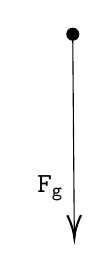
\begin{tikzpicture}[x=0.75pt,y=0.75pt,yscale=-1,xscale=1]
%uncomment if require: \path (0,300); %set diagram left start at 0, and has height of 300

%Shape: Circle [id:dp6401125961176861] 
\draw  [fill={rgb, 255:red, 0; green, 0; blue, 0 }  ,fill opacity=1 ] (330.88,127.88) .. controls (330.88,126.29) and (332.16,125) .. (333.75,125) .. controls (335.34,125) and (336.63,126.29) .. (336.63,127.88) .. controls (336.63,129.46) and (335.34,130.75) .. (333.75,130.75) .. controls (332.16,130.75) and (330.88,129.46) .. (330.88,127.88) -- cycle ;
%Straight Lines [id:da01700580379156591] 
\draw    (333.75,130.75) -- (334.48,224) ;
\draw [shift={(334.5,226)}, rotate = 269.55] [color={rgb, 255:red, 0; green, 0; blue, 0 }  ][line width=0.75]    (10.93,-3.29) .. controls (6.95,-1.4) and (3.31,-0.3) .. (0,0) .. controls (3.31,0.3) and (6.95,1.4) .. (10.93,3.29)   ;

% Text Node
\draw (323,202) node   [align=left] {F\textsubscript{g}};


\end{tikzpicture}

\end{center}
    \caption{Forces on the Spring}
\end{figure}

Because the gravitational force is acting against the restoring force, it can be found that:

$$F_g = -F_s$$

It can then be substituted:

$$F_s = -k\Delta x \longrightarrow -F_g = -k\Delta x \longrightarrow mg = k\Delta x$$
\vspace{16pt}
Here is a sample calculation:\\
\vspace{8pt}
When a 1[$\si{\kilo\gram}$] weight is hung from the spring, the displacement is 21.5[$\si{\centi\meter}$], or .215[$\si{\meter}$]. When plugged into the formula, it is obtained that:

$$g = k*.215[\si{\meter}]\longrightarrow\frac{g}{.215} = k$$
$$\therefore k = 45.612\left[\si{\frac{\newton}{\meter}}\right]$$

To plot this a function, with slope $k$, it can be re-arranged as shown:

$$mg = kx \longrightarrow m = \frac{kx}{g} \longrightarrow m = \frac{kx}{9.80665\left[\si{\frac{\meter}{\square\second}}}\right]$$

The graph would then need to have the mass as the vertical axis, and $\frac{x}{g}$ as the horizontal axis, to yield $k$ as the slope. (Figure 3)
\subsubsection{Graphing}

\begin{figure}[H]
    \centering
    \includegraphics[width=.75\columnwidth]{Slide2}
    \caption{Mass versus Displacemet over Gravitational Acceleration}
\end{figure}

\newpage
\subsection{Method 2}
\begin{figure}[H]
    
\begin{center}

\tikzset{every picture/.style={line width=0.75pt}} %set default line width to 0.75pt        

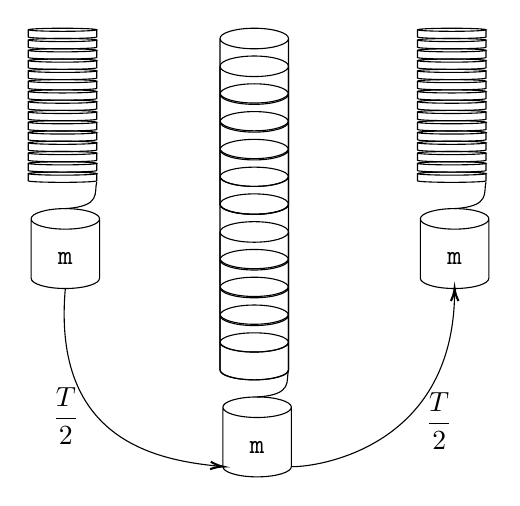
\begin{tikzpicture}[x=0.75pt,y=0.75pt,yscale=-.55,xscale=.55]
%uncomment if require: \path (0,431); %set diagram left start at 0, and has height of 431

%Shape: Can [id:dp5872210600345684] 
\draw   (268,29) -- (268,76.53) .. controls (268,81.5) and (254.57,85.53) .. (238,85.53) .. controls (221.43,85.53) and (208,81.5) .. (208,76.53) -- (208,29) .. controls (208,24.03) and (221.43,20) .. (238,20) .. controls (254.57,20) and (268,24.03) .. (268,29) .. controls (268,33.97) and (254.57,38) .. (238,38) .. controls (221.43,38) and (208,33.97) .. (208,29) ;
%Shape: Can [id:dp07537248954513087] 
\draw   (268,150.13) -- (268,174.47) .. controls (268,179.12) and (254.57,182.89) .. (238,182.89) .. controls (221.43,182.89) and (208,179.12) .. (208,174.47) -- (208,150.13) .. controls (208,145.47) and (221.43,141.7) .. (238,141.7) .. controls (254.57,141.7) and (268,145.47) .. (268,150.13) .. controls (268,154.78) and (254.57,158.55) .. (238,158.55) .. controls (221.43,158.55) and (208,154.78) .. (208,150.13) ;
%Shape: Can [id:dp6030545381327717] 
\draw   (268,77.68) -- (268,125.21) .. controls (268,130.18) and (254.57,134.21) .. (238,134.21) .. controls (221.43,134.21) and (208,130.18) .. (208,125.21) -- (208,77.68) .. controls (208,72.71) and (221.43,68.68) .. (238,68.68) .. controls (254.57,68.68) and (268,72.71) .. (268,77.68) .. controls (268,82.65) and (254.57,86.68) .. (238,86.68) .. controls (221.43,86.68) and (208,82.65) .. (208,77.68) ;
%Shape: Can [id:dp2321627970178879] 
\draw   (268,53.34) -- (268,100.87) .. controls (268,105.84) and (254.57,109.87) .. (238,109.87) .. controls (221.43,109.87) and (208,105.84) .. (208,100.87) -- (208,53.34) .. controls (208,48.37) and (221.43,44.34) .. (238,44.34) .. controls (254.57,44.34) and (268,48.37) .. (268,53.34) .. controls (268,58.31) and (254.57,62.34) .. (238,62.34) .. controls (221.43,62.34) and (208,58.31) .. (208,53.34) ;
%Shape: Can [id:dp5192692456190116] 
\draw   (268,102.02) -- (268,149.55) .. controls (268,154.52) and (254.57,158.55) .. (238,158.55) .. controls (221.43,158.55) and (208,154.52) .. (208,149.55) -- (208,102.02) .. controls (208,97.05) and (221.43,93.02) .. (238,93.02) .. controls (254.57,93.02) and (268,97.05) .. (268,102.02) .. controls (268,106.99) and (254.57,111.02) .. (238,111.02) .. controls (221.43,111.02) and (208,106.99) .. (208,102.02) ;
%Shape: Can [id:dp2130085867942586] 
\draw   (268,126.36) -- (268,173.89) .. controls (268,178.86) and (254.57,182.89) .. (238,182.89) .. controls (221.43,182.89) and (208,178.86) .. (208,173.89) -- (208,126.36) .. controls (208,121.39) and (221.43,117.36) .. (238,117.36) .. controls (254.57,117.36) and (268,121.39) .. (268,126.36) .. controls (268,131.33) and (254.57,135.36) .. (238,135.36) .. controls (221.43,135.36) and (208,131.33) .. (208,126.36) ;

%Shape: Can [id:dp8317637504092867] 
\draw   (268,174.11) -- (268,221.64) .. controls (268,226.61) and (254.57,230.64) .. (238,230.64) .. controls (221.43,230.64) and (208,226.61) .. (208,221.64) -- (208,174.11) .. controls (208,169.14) and (221.43,165.11) .. (238,165.11) .. controls (254.57,165.11) and (268,169.14) .. (268,174.11) .. controls (268,179.08) and (254.57,183.11) .. (238,183.11) .. controls (221.43,183.11) and (208,179.08) .. (208,174.11) ;
%Shape: Can [id:dp18280076747728646] 
\draw   (268,295.23) -- (268,319.57) .. controls (268,324.23) and (254.57,328) .. (238,328) .. controls (221.43,328) and (208,324.23) .. (208,319.57) -- (208,295.23) .. controls (208,290.58) and (221.43,286.81) .. (238,286.81) .. controls (254.57,286.81) and (268,290.58) .. (268,295.23) .. controls (268,299.89) and (254.57,303.66) .. (238,303.66) .. controls (221.43,303.66) and (208,299.89) .. (208,295.23) ;
%Shape: Can [id:dp9862426548941483] 
\draw   (268,222.79) -- (268,270.32) .. controls (268,275.29) and (254.57,279.32) .. (238,279.32) .. controls (221.43,279.32) and (208,275.29) .. (208,270.32) -- (208,222.79) .. controls (208,217.82) and (221.43,213.79) .. (238,213.79) .. controls (254.57,213.79) and (268,217.82) .. (268,222.79) .. controls (268,227.76) and (254.57,231.79) .. (238,231.79) .. controls (221.43,231.79) and (208,227.76) .. (208,222.79) ;
%Shape: Can [id:dp9742214883747009] 
\draw   (268,198.45) -- (268,245.98) .. controls (268,250.95) and (254.57,254.98) .. (238,254.98) .. controls (221.43,254.98) and (208,250.95) .. (208,245.98) -- (208,198.45) .. controls (208,193.48) and (221.43,189.45) .. (238,189.45) .. controls (254.57,189.45) and (268,193.48) .. (268,198.45) .. controls (268,203.42) and (254.57,207.45) .. (238,207.45) .. controls (221.43,207.45) and (208,203.42) .. (208,198.45) ;
%Shape: Can [id:dp29099849582792414] 
\draw   (268,247.13) -- (268,294.66) .. controls (268,299.63) and (254.57,303.66) .. (238,303.66) .. controls (221.43,303.66) and (208,299.63) .. (208,294.66) -- (208,247.13) .. controls (208,242.16) and (221.43,238.13) .. (238,238.13) .. controls (254.57,238.13) and (268,242.16) .. (268,247.13) .. controls (268,252.1) and (254.57,256.13) .. (238,256.13) .. controls (221.43,256.13) and (208,252.1) .. (208,247.13) ;
%Shape: Can [id:dp6195165542280063] 
\draw   (268,271.47) -- (268,319) .. controls (268,323.97) and (254.57,328) .. (238,328) .. controls (221.43,328) and (208,323.97) .. (208,319) -- (208,271.47) .. controls (208,266.5) and (221.43,262.47) .. (238,262.47) .. controls (254.57,262.47) and (268,266.5) .. (268,271.47) .. controls (268,276.44) and (254.57,280.47) .. (238,280.47) .. controls (221.43,280.47) and (208,276.44) .. (208,271.47) ;


%Curve Lines [id:da711884872517422] 
\draw    (268,319.57) .. controls (265.5,329) and (272.5,341) .. (240.5,343) ;
%Shape: Can [id:dp8371864574267989] 
\draw   (270.5,352) -- (270.5,404) .. controls (270.5,408.97) and (257.07,413) .. (240.5,413) .. controls (223.93,413) and (210.5,408.97) .. (210.5,404) -- (210.5,352) .. controls (210.5,347.03) and (223.93,343) .. (240.5,343) .. controls (257.07,343) and (270.5,347.03) .. (270.5,352) .. controls (270.5,356.97) and (257.07,361) .. (240.5,361) .. controls (223.93,361) and (210.5,356.97) .. (210.5,352) ;

%Shape: Can [id:dp6395199666701763] 
\draw   (100,21.35) -- (100,27.65) .. controls (100,28.4) and (86.57,29) .. (70,29) .. controls (53.43,29) and (40,28.4) .. (40,27.65) -- (40,21.35) .. controls (40,20.6) and (53.43,20) .. (70,20) .. controls (86.57,20) and (100,20.6) .. (100,21.35) .. controls (100,22.1) and (86.57,22.7) .. (70,22.7) .. controls (53.43,22.7) and (40,22.1) .. (40,21.35) ;
%Shape: Can [id:dp8792772347143301] 
\draw   (100,30.35) -- (100,36.65) .. controls (100,37.4) and (86.57,38) .. (70,38) .. controls (53.43,38) and (40,37.4) .. (40,36.65) -- (40,30.35) .. controls (40,29.6) and (53.43,29) .. (70,29) .. controls (86.57,29) and (100,29.6) .. (100,30.35) .. controls (100,31.1) and (86.57,31.7) .. (70,31.7) .. controls (53.43,31.7) and (40,31.1) .. (40,30.35) ;
%Shape: Can [id:dp25408387353719686] 
\draw   (100,39.35) -- (100,45.65) .. controls (100,46.4) and (86.57,47) .. (70,47) .. controls (53.43,47) and (40,46.4) .. (40,45.65) -- (40,39.35) .. controls (40,38.6) and (53.43,38) .. (70,38) .. controls (86.57,38) and (100,38.6) .. (100,39.35) .. controls (100,40.1) and (86.57,40.7) .. (70,40.7) .. controls (53.43,40.7) and (40,40.1) .. (40,39.35) ;
%Shape: Can [id:dp6721535977010693] 
\draw   (100,48.35) -- (100,54.65) .. controls (100,55.4) and (86.57,56) .. (70,56) .. controls (53.43,56) and (40,55.4) .. (40,54.65) -- (40,48.35) .. controls (40,47.6) and (53.43,47) .. (70,47) .. controls (86.57,47) and (100,47.6) .. (100,48.35) .. controls (100,49.1) and (86.57,49.7) .. (70,49.7) .. controls (53.43,49.7) and (40,49.1) .. (40,48.35) ;
%Shape: Can [id:dp4757014014139824] 
\draw   (100,57.35) -- (100,63.65) .. controls (100,64.4) and (86.57,65) .. (70,65) .. controls (53.43,65) and (40,64.4) .. (40,63.65) -- (40,57.35) .. controls (40,56.6) and (53.43,56) .. (70,56) .. controls (86.57,56) and (100,56.6) .. (100,57.35) .. controls (100,58.1) and (86.57,58.7) .. (70,58.7) .. controls (53.43,58.7) and (40,58.1) .. (40,57.35) ;
%Shape: Can [id:dp2810915196899151] 
\draw   (100,66.35) -- (100,72.65) .. controls (100,73.4) and (86.57,74) .. (70,74) .. controls (53.43,74) and (40,73.4) .. (40,72.65) -- (40,66.35) .. controls (40,65.6) and (53.43,65) .. (70,65) .. controls (86.57,65) and (100,65.6) .. (100,66.35) .. controls (100,67.1) and (86.57,67.7) .. (70,67.7) .. controls (53.43,67.7) and (40,67.1) .. (40,66.35) ;
%Shape: Can [id:dp4680636273134806] 
\draw   (100,75.35) -- (100,81.65) .. controls (100,82.4) and (86.57,83) .. (70,83) .. controls (53.43,83) and (40,82.4) .. (40,81.65) -- (40,75.35) .. controls (40,74.6) and (53.43,74) .. (70,74) .. controls (86.57,74) and (100,74.6) .. (100,75.35) .. controls (100,76.1) and (86.57,76.7) .. (70,76.7) .. controls (53.43,76.7) and (40,76.1) .. (40,75.35) ;
%Shape: Can [id:dp2207486669731058] 
\draw   (100,84.35) -- (100,90.65) .. controls (100,91.4) and (86.57,92) .. (70,92) .. controls (53.43,92) and (40,91.4) .. (40,90.65) -- (40,84.35) .. controls (40,83.6) and (53.43,83) .. (70,83) .. controls (86.57,83) and (100,83.6) .. (100,84.35) .. controls (100,85.1) and (86.57,85.7) .. (70,85.7) .. controls (53.43,85.7) and (40,85.1) .. (40,84.35) ;
%Shape: Can [id:dp5449621401848834] 
\draw   (100,93.35) -- (100,99.65) .. controls (100,100.4) and (86.57,101) .. (70,101) .. controls (53.43,101) and (40,100.4) .. (40,99.65) -- (40,93.35) .. controls (40,92.6) and (53.43,92) .. (70,92) .. controls (86.57,92) and (100,92.6) .. (100,93.35) .. controls (100,94.1) and (86.57,94.7) .. (70,94.7) .. controls (53.43,94.7) and (40,94.1) .. (40,93.35) ;
%Shape: Can [id:dp33551965974876863] 
\draw   (100,102.35) -- (100,108.65) .. controls (100,109.4) and (86.57,110) .. (70,110) .. controls (53.43,110) and (40,109.4) .. (40,108.65) -- (40,102.35) .. controls (40,101.6) and (53.43,101) .. (70,101) .. controls (86.57,101) and (100,101.6) .. (100,102.35) .. controls (100,103.1) and (86.57,103.7) .. (70,103.7) .. controls (53.43,103.7) and (40,103.1) .. (40,102.35) ;
%Shape: Can [id:dp3495672378256558] 
\draw   (100,111.35) -- (100,117.65) .. controls (100,118.4) and (86.57,119) .. (70,119) .. controls (53.43,119) and (40,118.4) .. (40,117.65) -- (40,111.35) .. controls (40,110.6) and (53.43,110) .. (70,110) .. controls (86.57,110) and (100,110.6) .. (100,111.35) .. controls (100,112.1) and (86.57,112.7) .. (70,112.7) .. controls (53.43,112.7) and (40,112.1) .. (40,111.35) ;
%Shape: Can [id:dp45057016599678246] 
\draw   (100,120.35) -- (100,126.65) .. controls (100,127.4) and (86.57,128) .. (70,128) .. controls (53.43,128) and (40,127.4) .. (40,126.65) -- (40,120.35) .. controls (40,119.6) and (53.43,119) .. (70,119) .. controls (86.57,119) and (100,119.6) .. (100,120.35) .. controls (100,121.1) and (86.57,121.7) .. (70,121.7) .. controls (53.43,121.7) and (40,121.1) .. (40,120.35) ;
%Shape: Can [id:dp6587457072568552] 
\draw   (100,129.35) -- (100,135.65) .. controls (100,136.4) and (86.57,137) .. (70,137) .. controls (53.43,137) and (40,136.4) .. (40,135.65) -- (40,129.35) .. controls (40,128.6) and (53.43,128) .. (70,128) .. controls (86.57,128) and (100,128.6) .. (100,129.35) .. controls (100,130.1) and (86.57,130.7) .. (70,130.7) .. controls (53.43,130.7) and (40,130.1) .. (40,129.35) ;
%Shape: Can [id:dp31633049761964016] 
\draw   (100,138.35) -- (100,144.65) .. controls (100,145.4) and (86.57,146) .. (70,146) .. controls (53.43,146) and (40,145.4) .. (40,144.65) -- (40,138.35) .. controls (40,137.6) and (53.43,137) .. (70,137) .. controls (86.57,137) and (100,137.6) .. (100,138.35) .. controls (100,139.1) and (86.57,139.7) .. (70,139.7) .. controls (53.43,139.7) and (40,139.1) .. (40,138.35) ;
%Shape: Can [id:dp45947820598785816] 
\draw   (100,147.35) -- (100,153.65) .. controls (100,154.4) and (86.57,155) .. (70,155) .. controls (53.43,155) and (40,154.4) .. (40,153.65) -- (40,147.35) .. controls (40,146.6) and (53.43,146) .. (70,146) .. controls (86.57,146) and (100,146.6) .. (100,147.35) .. controls (100,148.1) and (86.57,148.7) .. (70,148.7) .. controls (53.43,148.7) and (40,148.1) .. (40,147.35) ;

%Curve Lines [id:da5371000587168375] 
\draw    (100,154.57) .. controls (97.5,164) and (104.5,176) .. (72.5,178) ;
%Shape: Can [id:dp817396419005834] 
\draw   (102.5,187) -- (102.5,239) .. controls (102.5,243.97) and (89.07,248) .. (72.5,248) .. controls (55.93,248) and (42.5,243.97) .. (42.5,239) -- (42.5,187) .. controls (42.5,182.03) and (55.93,178) .. (72.5,178) .. controls (89.07,178) and (102.5,182.03) .. (102.5,187) .. controls (102.5,191.97) and (89.07,196) .. (72.5,196) .. controls (55.93,196) and (42.5,191.97) .. (42.5,187) ;


%Shape: Can [id:dp26680088965465565] 
\draw   (441,21.35) -- (441,27.65) .. controls (441,28.4) and (427.57,29) .. (411,29) .. controls (394.43,29) and (381,28.4) .. (381,27.65) -- (381,21.35) .. controls (381,20.6) and (394.43,20) .. (411,20) .. controls (427.57,20) and (441,20.6) .. (441,21.35) .. controls (441,22.1) and (427.57,22.7) .. (411,22.7) .. controls (394.43,22.7) and (381,22.1) .. (381,21.35) ;
%Shape: Can [id:dp9806657637578318] 
\draw   (441,30.35) -- (441,36.65) .. controls (441,37.4) and (427.57,38) .. (411,38) .. controls (394.43,38) and (381,37.4) .. (381,36.65) -- (381,30.35) .. controls (381,29.6) and (394.43,29) .. (411,29) .. controls (427.57,29) and (441,29.6) .. (441,30.35) .. controls (441,31.1) and (427.57,31.7) .. (411,31.7) .. controls (394.43,31.7) and (381,31.1) .. (381,30.35) ;
%Shape: Can [id:dp3850047429115002] 
\draw   (441,39.35) -- (441,45.65) .. controls (441,46.4) and (427.57,47) .. (411,47) .. controls (394.43,47) and (381,46.4) .. (381,45.65) -- (381,39.35) .. controls (381,38.6) and (394.43,38) .. (411,38) .. controls (427.57,38) and (441,38.6) .. (441,39.35) .. controls (441,40.1) and (427.57,40.7) .. (411,40.7) .. controls (394.43,40.7) and (381,40.1) .. (381,39.35) ;
%Shape: Can [id:dp4104874062299886] 
\draw   (441,48.35) -- (441,54.65) .. controls (441,55.4) and (427.57,56) .. (411,56) .. controls (394.43,56) and (381,55.4) .. (381,54.65) -- (381,48.35) .. controls (381,47.6) and (394.43,47) .. (411,47) .. controls (427.57,47) and (441,47.6) .. (441,48.35) .. controls (441,49.1) and (427.57,49.7) .. (411,49.7) .. controls (394.43,49.7) and (381,49.1) .. (381,48.35) ;
%Shape: Can [id:dp05050993312788066] 
\draw   (441,57.35) -- (441,63.65) .. controls (441,64.4) and (427.57,65) .. (411,65) .. controls (394.43,65) and (381,64.4) .. (381,63.65) -- (381,57.35) .. controls (381,56.6) and (394.43,56) .. (411,56) .. controls (427.57,56) and (441,56.6) .. (441,57.35) .. controls (441,58.1) and (427.57,58.7) .. (411,58.7) .. controls (394.43,58.7) and (381,58.1) .. (381,57.35) ;
%Shape: Can [id:dp38408863901005286] 
\draw   (441,66.35) -- (441,72.65) .. controls (441,73.4) and (427.57,74) .. (411,74) .. controls (394.43,74) and (381,73.4) .. (381,72.65) -- (381,66.35) .. controls (381,65.6) and (394.43,65) .. (411,65) .. controls (427.57,65) and (441,65.6) .. (441,66.35) .. controls (441,67.1) and (427.57,67.7) .. (411,67.7) .. controls (394.43,67.7) and (381,67.1) .. (381,66.35) ;
%Shape: Can [id:dp3604005812641953] 
\draw   (441,75.35) -- (441,81.65) .. controls (441,82.4) and (427.57,83) .. (411,83) .. controls (394.43,83) and (381,82.4) .. (381,81.65) -- (381,75.35) .. controls (381,74.6) and (394.43,74) .. (411,74) .. controls (427.57,74) and (441,74.6) .. (441,75.35) .. controls (441,76.1) and (427.57,76.7) .. (411,76.7) .. controls (394.43,76.7) and (381,76.1) .. (381,75.35) ;
%Shape: Can [id:dp2637816060300475] 
\draw   (441,84.35) -- (441,90.65) .. controls (441,91.4) and (427.57,92) .. (411,92) .. controls (394.43,92) and (381,91.4) .. (381,90.65) -- (381,84.35) .. controls (381,83.6) and (394.43,83) .. (411,83) .. controls (427.57,83) and (441,83.6) .. (441,84.35) .. controls (441,85.1) and (427.57,85.7) .. (411,85.7) .. controls (394.43,85.7) and (381,85.1) .. (381,84.35) ;
%Shape: Can [id:dp46438722738478844] 
\draw   (441,93.35) -- (441,99.65) .. controls (441,100.4) and (427.57,101) .. (411,101) .. controls (394.43,101) and (381,100.4) .. (381,99.65) -- (381,93.35) .. controls (381,92.6) and (394.43,92) .. (411,92) .. controls (427.57,92) and (441,92.6) .. (441,93.35) .. controls (441,94.1) and (427.57,94.7) .. (411,94.7) .. controls (394.43,94.7) and (381,94.1) .. (381,93.35) ;
%Shape: Can [id:dp9204861962967159] 
\draw   (441,102.35) -- (441,108.65) .. controls (441,109.4) and (427.57,110) .. (411,110) .. controls (394.43,110) and (381,109.4) .. (381,108.65) -- (381,102.35) .. controls (381,101.6) and (394.43,101) .. (411,101) .. controls (427.57,101) and (441,101.6) .. (441,102.35) .. controls (441,103.1) and (427.57,103.7) .. (411,103.7) .. controls (394.43,103.7) and (381,103.1) .. (381,102.35) ;
%Shape: Can [id:dp3191697359793182] 
\draw   (441,111.35) -- (441,117.65) .. controls (441,118.4) and (427.57,119) .. (411,119) .. controls (394.43,119) and (381,118.4) .. (381,117.65) -- (381,111.35) .. controls (381,110.6) and (394.43,110) .. (411,110) .. controls (427.57,110) and (441,110.6) .. (441,111.35) .. controls (441,112.1) and (427.57,112.7) .. (411,112.7) .. controls (394.43,112.7) and (381,112.1) .. (381,111.35) ;
%Shape: Can [id:dp18426413332476033] 
\draw   (441,120.35) -- (441,126.65) .. controls (441,127.4) and (427.57,128) .. (411,128) .. controls (394.43,128) and (381,127.4) .. (381,126.65) -- (381,120.35) .. controls (381,119.6) and (394.43,119) .. (411,119) .. controls (427.57,119) and (441,119.6) .. (441,120.35) .. controls (441,121.1) and (427.57,121.7) .. (411,121.7) .. controls (394.43,121.7) and (381,121.1) .. (381,120.35) ;
%Shape: Can [id:dp6821996943224939] 
\draw   (441,129.35) -- (441,135.65) .. controls (441,136.4) and (427.57,137) .. (411,137) .. controls (394.43,137) and (381,136.4) .. (381,135.65) -- (381,129.35) .. controls (381,128.6) and (394.43,128) .. (411,128) .. controls (427.57,128) and (441,128.6) .. (441,129.35) .. controls (441,130.1) and (427.57,130.7) .. (411,130.7) .. controls (394.43,130.7) and (381,130.1) .. (381,129.35) ;
%Shape: Can [id:dp4356686985283298] 
\draw   (441,138.35) -- (441,144.65) .. controls (441,145.4) and (427.57,146) .. (411,146) .. controls (394.43,146) and (381,145.4) .. (381,144.65) -- (381,138.35) .. controls (381,137.6) and (394.43,137) .. (411,137) .. controls (427.57,137) and (441,137.6) .. (441,138.35) .. controls (441,139.1) and (427.57,139.7) .. (411,139.7) .. controls (394.43,139.7) and (381,139.1) .. (381,138.35) ;
%Shape: Can [id:dp19632565387539858] 
\draw   (441,147.35) -- (441,153.65) .. controls (441,154.4) and (427.57,155) .. (411,155) .. controls (394.43,155) and (381,154.4) .. (381,153.65) -- (381,147.35) .. controls (381,146.6) and (394.43,146) .. (411,146) .. controls (427.57,146) and (441,146.6) .. (441,147.35) .. controls (441,148.1) and (427.57,148.7) .. (411,148.7) .. controls (394.43,148.7) and (381,148.1) .. (381,147.35) ;

%Curve Lines [id:da9275038767667361] 
\draw    (441,154.57) .. controls (438.5,164) and (445.5,176) .. (413.5,178) ;
%Shape: Can [id:dp34114981711853676] 
\draw   (443.5,187) -- (443.5,239) .. controls (443.5,243.97) and (430.07,248) .. (413.5,248) .. controls (396.93,248) and (383.5,243.97) .. (383.5,239) -- (383.5,187) .. controls (383.5,182.03) and (396.93,178) .. (413.5,178) .. controls (430.07,178) and (443.5,182.03) .. (443.5,187) .. controls (443.5,191.97) and (430.07,196) .. (413.5,196) .. controls (396.93,196) and (383.5,191.97) .. (383.5,187) ;


%Curve Lines [id:da41381333764291695] 
\draw    (72.5,248) .. controls (60.62,382.64) and (154.59,398.69) .. (208.87,403.85) ;
\draw [shift={(210.5,404)}, rotate = 185.29] [color={rgb, 255:red, 0; green, 0; blue, 0 }  ][line width=0.75]    (10.93,-3.29) .. controls (6.95,-1.4) and (3.31,-0.3) .. (0,0) .. controls (3.31,0.3) and (6.95,1.4) .. (10.93,3.29)   ;
%Curve Lines [id:da6356030331449392] 
\draw    (413.51,250.15) .. controls (413.21,392.13) and (285.43,405) .. (270.5,404) ;
\draw [shift={(413.5,248)}, rotate = 89.6] [color={rgb, 255:red, 0; green, 0; blue, 0 }  ][line width=0.75]    (10.93,-3.29) .. controls (6.95,-1.4) and (3.31,-0.3) .. (0,0) .. controls (3.31,0.3) and (6.95,1.4) .. (10.93,3.29)   ;

% Text Node
\draw (72.5,222) node   [align=left] {m};
% Text Node
\draw (240.5,387) node   [align=left] {m};
% Text Node
\draw (413.5,222) node   [align=left] {m};
% Text Node
\draw (73,360) node   [align=left] {$\displaystyle \frac{T}{2}$};
% Text Node
\draw (400,364) node   [align=left] {$\displaystyle \frac{T}{2}$};


\end{tikzpicture}
\end{center}
    \caption{The Spring Oscillates with Mass, $m$}
\end{figure}

\subsubsection{Data Table}
\begin{center}
\begin{tabular}{|c|c|}
\hline
    Mass [$\si{\kilo\gram}$] & Period [$\si{\second}$]\\
\hline
    1 & .97\\
\hline
    .75 & .84\\
\hline
    .5 & .75 \\
\hline
    .4 & .61 \\
\hline
    .2 & .5 \\
\hline
\end{tabular}
\end{center}

\subsubsection{Experimentation Process}

\begin{enumerate}
    
    \item Set up the spring as shown in figure 4
    
    \item Compress the mass and spring slightly, then let go
    
    \item Record the spring in a slow motion video 
    
    \item Use the video to find the period (one full up and down motion)
    
    \item Implement the formula below
    
\end{enumerate}


\subsubsection{Formulation}
According to the model above (Figure 4), a timer will be used to approximate the period, $T$, of the spring and mass.
The formula to determine the spring constant, $k$, with the period, $T$, and mass, $m$ is:

$$T = 2\pi\sqrt{\frac{m}{k}}$$

This can be re-arranged to yield the slope formula:

$$\frac{4\pi^2}{T^2}=\frac{k}{m}$$

This means that the vertical axis is $\frac{4\pi^2}{T^2}$, the horizontal axis is $\frac{1}{m}$, and the slope is $k$. (Figure 5)

\subsubsection{Graphing}

\begin{figure}[H]
\centering
    \includegraphics[width=.75\columnwidth]{Slide1}
    \caption{Four $\pi^2$ Times Inverse Square Period versus Inverse Mass }
\end{figure}

\newpage
\subsection{Conclusion}

\subsubsection{Margin of Error}

The graph for the Hooke's law method (figure 3) yields 42.96 $\left[\si{\frac{\newton}{\meter}}\right]$ as the spring constant.\\
The graph for the second method (figure 5) yields 39.70 $\left[\si{\frac{\newton}{\meter}}\right]$ as the spring constant.\\

\flushleft The percent difference can be found using $\frac{|42.96-39.70|}{(42.96 + 39.70)/2} * 100\%$\\
This is approximately equal to: 7.888\%


\subsubsection{Which Method is More Accurate?}

Most likely, Hooke's law would be the most accurate. This is because the second method depends on the analysis of a slow motion video, and, as such, is subject to significant human error. Such a fatal error would render the results inconclusive, whereas the stationary spring method has little to no possible human error. Therefore, the displacement method was more accurate


\subsubsection{Error Analysis}
\begin{enumerate}

    \item \textsc{Spring Use} $-$ With use, the springs will have a greater stretch property. This use can result in an ever-changing spring constant. Because the spring is stretching, the spring constant would be constantly decreasing with use, and the correct spring constant will change with each use. (Affects both methods)
    
    \item \textsc{Frictional Forces} $-$ During the simple harmonic motion of the spring, there exist frictional forces due to the motion through the medium (in this case, air). These forces would cause a deceleration in the motion of the spring, and therefore an increasing period. These errors can, however, be nullified by recording a certain period for each repetition of the experiment. For example, one would agree to use the first period after the spring is set in motion. (Affects method 2)
    
\end{enumerate}

\subsubsection{Finding the Mass of an Unknown Object}

To find the mass of an unknown object requires the spring constant. This can be found by using a known mass, coupled with one of the above methods. Once the spring constant is determined, once again use one of the above methods, now with the unknown object. For example, if one used Hooke's law, the setup for mass would be:

$$m = \frac{k\Delta x}{g}$$









\end{document}
